\documentclass[11pt,handout,aspectratio=169]{beamer}


%%%%%%%%% GENERAL PACKAGES
%\usepackage{xcolor}
%\usepackage{pdfpages}
%\usetheme[progressbar=frametitle]{metropolis}
%\setbeamercolor{background canvas}{bg=white}
%\usepackage{appendixnumberbeamer}
%\usepackage{booktabs}
%\usepackage[scale=2]{ccicons}
%\usepackage{pgfplots}
%\usepgfplotslibrary{dateplot}
%\usepackage{xspace}
%\newcommand{\themename}{\textbf{\textsc{metropolis}}\xspace}
%\usepackage[absolute,overlay]{textpos}

%%%%%%%%% COLOR THEME

% Define some colors:
\definecolor{DarkFern}{HTML}{407428}
\definecolor{DarkCharcoal}{HTML}{4D4944}
\definecolor{AlertColor}{RGB}{89,124,158}
\definecolor{HighLight}{RGB}{96,95,134}
\definecolor{Important}{RGB}{234,122,133}
\definecolor{Yellow}{HTML}{00539C}
\colorlet{Fern}{DarkFern!85!white}
\colorlet{Charcoal}{DarkCharcoal!85!white}
\colorlet{LightCharcoal}{Charcoal!50!white}
\colorlet{HighLight2}{AlertColor}
\colorlet{DarkRed}{red!70!black}
\colorlet{DarkBlue}{blue!70!black}
\colorlet{DarkGreen}{green!70!black}
\definecolor{RoyalBlue}{HTML}{00539C}
\definecolor{Peach}{HTML}{EEA47F}
\definecolor{ForestGreen}{HTML}{2C5F2D}
\definecolor{MossGreen}{HTML}{E8FCC9}
% Use the colors:
\setbeamercolor{title}{fg=Fern}
\setbeamercolor{frametitle}{fg=MossGreen,bg=ForestGreen}
\setbeamercolor{normal text}{fg=Charcoal!70!black}
\setbeamercolor{block title}{fg=black,bg=Fern!25!white}
\setbeamercolor{block body}{fg=black,bg=Fern!10!white}
\setbeamercolor{block title alerted}{fg=black,bg=DarkRed!25!white}
\setbeamercolor{block body alerted}{fg=black,bg=DarkRed!10!white}
\setbeamercolor{alerted text}{fg=DarkRed}
\setbeamercolor{itemize item}{fg=Charcoal}



%%%%%%%%% OTHER COMMANDS
\newcommand{\indep}{\perp\!\!\! \perp}
\newcommand{\comment}[1]{}
\newcommand{\bs}{\boldsymbol}
\newcommand{\tr}{\text{trace}}
\newcommand{\sgn}{{\rm sgn}}
\def\T{\top}
%\newcommand{\det}{\text{det}}
\newcommand{\var}{\mathrm{var}}
\newcommand{\cC}{{\cal C}}
\newcommand{\cG}{{\cal G}}
\newcommand{\cV}{{\cal V}}
\newcommand{\cE}{{\cal E}}
\newcommand{\cM}{{\cal M}}
\newcommand{\cP}{{\cal P}}
\newcommand{\cX}{{\cal X}}
\newcommand{\cY}{{\cal Y}}
\newcommand{\X}{\mathbf{X}}
\newcommand{\Y}{\mathbf{Y}}
\newcommand{\x}{\mathbf{x}}
\newcommand{\y}{\mathbf{y}}
\newcommand{\z}{\mathbf{z}}

\newcommand{\argmin}{\operatornamewithlimits{argmin}}
\newcommand{\eps}{\varepsilon}
\newcommand{\<}{\langle}
\renewcommand{\>}{\rangle}


\setbeamertemplate{itemize subitem}{\tiny\raise1.5pt\hbox{\donotcoloroutermaths$\blacktriangleright$}}
\setbeamertemplate{itemize subsubitem}{\tiny\raise1.5pt\hbox{\donotcoloroutermaths$\blacktriangleright$}}
\setbeamertemplate{enumerate item}{\insertenumlabel.}
\setbeamertemplate{enumerate subitem}{\insertenumlabel.\insertsubenumlabel}
\setbeamertemplate{enumerate subsubitem}{\insertenumlabel.\insertsubenumlabel.\insertsubsubenumlabel}
\setbeamertemplate{enumerate mini template}{\insertenumlabel}

\newcommand{\TODO}[1]{{\color{red}{[TODO: #1]}}}


\newcommand{\R}{\mathbb R}
\newcommand{\E}{\mathbb E}
\renewcommand{\P}{\mathbb P}


\DeclareMathOperator*{\cov}{cov}


\newsavebox{\zerobox}
\newenvironment{nospace}
{\par\edef\theprevdepth{\the\prevdepth}\nointerlineskip
  \setbox\zerobox=\vtop to 0pt\bgroup
  \hrule height0pt\kern\dimexpr\baselineskip-\topskip\relax
}
{\par\vss\egroup\ht\zerobox=0pt \wd\zerobox=0pt \dp\zerobox=0pt
  \box\zerobox}

\usepackage{soul}
\makeatletter
\let\HL\hl
\renewcommand\hl{%
  \let\set@color\beamerorig@set@color
  \let\reset@color\beamerorig@reset@color
  \HL}
  \makeatother


\title[STA437-Week1]{STA 437/2005: \\ Methods for Multivariate Data}
\subtitle[]{Week 1: Introduction and Preliminaries}
\author[Prob Learning]{Piotr Zwiernik}
\institute[UofT]{University of Toronto}
\date{}


\usepackage{Sweave}


\begin{document}

\maketitle

\begin{frame}{Table of contents}
  \setbeamertemplate{section in toc}[sections numbered]
  \tableofcontents%[hideallsubsections]
\end{frame}



\section{What is this class about?}
% \begin{frame}
% {The Team I}


\begin{frame}{Multivariate datasets}
\begin{itemize}
	\item Modern datasets are high-dimensional and highly unstructured.\\[.7cm]
	\item This means that we simultaneously observe many correlated features. \\[.7cm]
	\item Modelling them independently is \emph{wasteful}.\\[.7cm]
	\item Modelling them jointly is \emph{hard}!\\[.7cm]
	\item Our intuition works well only in 1D-3D so we need to develop tools to guide it.
\end{itemize}	
\end{frame}

\begin{frame}{This course}
  \begin{itemize}
  \item Discuss some classical and more modern methods for multivariate datasets.\begin{itemize}
  	\item Tentative outline of the course on the website\\[.7cm]
  \end{itemize}
  \item Build math toolbox that gives deeper understanding for these methods.\\[.7cm]
  \item Aimed at advanced undergrad and master level graduate students. \\[.7cm]
  \item 2 hrs lecture + 1 hour tutorial to get more hands-on experience. \\[.7cm]
  \item We will use \alert{a lot of} real analysis, probability, and linear algebra. 
  \begin{itemize}
\item To large extend I am assuming you are comfortable with matrix algebra. 
  \end{itemize}  
  \end{itemize}
\end{frame}


\section{Administrative details}
\begin{frame}{Course Information}
Course Website: \url{https://pzwiernik.github.io/sta437/} 

\vspace{.5em}
 % 
Main source of information is the course webpage; check regularly!

%\pause

We will also use \alert{Quercus} for { announcements \& grades}.

\begin{itemize}
\item You received an announcement on Sunday.
\end{itemize}
%\pause
 % 
We will use \alert{Piazza} for {discussions}.
\begin{itemize}
\item Sign up via quercus or: \url{https://piazza.com/utoronto.ca/winter2025/sta4372005}
\item Your grade { does not depend on your participation on Piazza}. 
\end{itemize}
\end{frame}



\begin{frame}{Course Information}
\begin{itemize}
\item This course have two \emph{identical} sections:
  \begin{itemize}
  \item Section 1: Wed 9-11am (tutorial Fri 9-10am)  
  \item Section 2: Wed 1-3pm (tutorial Fri 1-2pm)  
  \end{itemize}
\item You are welcome to attend either one of the sections.
  %\pause
\item Instructor office hours are on Tuesdays 13:30-15:00 (UY 9033).
%\pause
\item Questions during lectures/tutorials are always welcome!
\item The website contains the tentative schedule for the course and the dates of  all the course mark items (the final exam will be confirmed later). 
\end{itemize}
\end{frame}



\begin{frame}{Course Information}
  \begin{itemize}
  \item While cell phones and other electronics are not prohibited, recording or taking pictures in class is prohibited without the consent of your instructor.
  \item The lecture notes will cover everything presented in class. Let me know about typos you notice and/or any suggestions you might have.
  \item For accessibility services: If you require additional academic accommodations, please contact UofT Accessibility Services as soon as possible, \url{studentlife.utoronto.ca/as}. No last minute arrangements will be considered.   
  \end{itemize}
\end{frame}




%\begin{frame}[fragile]{Literature}
%This course is not following any particular book. \\[2mm]
%Recommended readings will be given for each lecture. The following will be useful throughout the course:
%{\small\begin{itemize} 
%\item Mardia, Kent, Bibby (1979), \textit{Multivariate Analysis}.
% \item  Everitt, Hothorn (2011), \textit{An Introduction to Applied Multivariate Analysis with R}. 
% \item Holms, Huber (2023), \textit{Modern Statistics for Modern Biology}.
%\end{itemize}}
%\bigskip 
%Some other books mentioned on the website.\\
%
%There are lots of freely available, high-quality resources online.
%
%\end{frame}

%\begin{frame}[Fragile]{Setup in R}
%<<>>=
%CRAN_pkgs <- c("ggplot2", "dplyr", "tidyr", "mosaicData",
%"carData", "VIM", "scales", "treemapify",
%"gapminder","sf", "tidygeocoder", "mapview",
%"ggmap", "osmdata", "choroplethr",
%"choroplethrMaps", "lubridate", "CGPfunctions",
%"ggcorrplot", "visreg", "gcookbook", "forcats",
%"survival", "survminer", "car", "rgl",
%"ggalluvial", "ggridges", "GGally", "superheat",
%"waterfalls", "factoextra","networkD3",
%"ggthemes", "patchwork", "hrbrthemes", "ggpol",
%"quantmod", "gghighlight", "leaflet", "ggiraph",
%"rbokeh", "ggalt","MVA")
%library(CRAN_pkgs)
%@	
%\end{frame}

\begin{frame}{Requirements and Marking}
\begin{itemize}
  \item Two midterms (conceptual/theoretical)
    \begin{itemize}
    \item 7 February and March 14 (tentative)
    \item $1$ hour tests 
    \item Worth 20\% of course mark each
    \end{itemize}
          %\pause
  \item Final projects
  \begin{itemize}
  	\item More details will be posted in the reading week.
  	\item 1-2 person groups
  	\item 20\% of course mark
  \end{itemize}
  \item Final Exam (conceptual/theoretical)
    \begin{itemize}
    \item $\sim 2$-$3$ hours
    \item Date and time TBA
    \item Worth 40\% of course mark
    \end{itemize}
    \item \alert{Everybody must take the final exam! No exceptions.}
  \end{itemize}
\end{frame}


\section{Introduction to multivariate statistics}

\begin{frame}{Multivariate data}
	\begin{itemize}
		\item Many datasets consist of several variables measured on the same set of subjects: patients, samples, users, or organisms.
		\item Goal: investigation of associations between the different variables measured.
		\item Usually the data are reported in a tabular data structure with one row for each subject and one column for each variable.  
	\end{itemize}
	\begin{exampleblock}{Example}
	Studying the expression of 25{,}000 gene (columns) on many samples (rows) of patient-derived cells, we notice that many of the genes act together, either that they are positively correlated or that they are anti-correlated. We would miss a lot of important information if we were to only study each gene separately.	
	\end{exampleblock}
\end{frame}

\begin{frame}[fragile]{Example 1: Decathlon}
The columns are the 10 disciplines in decathlon. The rows are the competitors:
{\scriptsize
\begin{Schunk}
\begin{Sinput}
> data("olympic", package = "ade4")
> athletes = setNames(olympic$tab, 
+   c("m100", "long", "weight", "high", "m400", "m110", "disc", "pole", "javel", "m1500"))
> head(athletes)
\end{Sinput}
\begin{Soutput}
   m100 long weight high  m400  m110  disc pole javel  m1500
1 11.25 7.43  15.48 2.27 48.90 15.13 49.28  4.7 61.32 268.95
2 10.87 7.45  14.97 1.97 47.71 14.46 44.36  5.1 61.76 273.02
3 11.18 7.44  14.20 1.97 48.29 14.81 43.66  5.2 64.16 263.20
4 10.62 7.38  15.02 2.03 49.06 14.72 44.80  4.9 64.04 285.11
5 11.02 7.43  12.92 1.97 47.44 14.40 41.20  5.2 57.46 256.64
6 10.83 7.72  13.58 2.12 48.34 14.18 43.06  4.9 52.18 274.07
\end{Soutput}
\end{Schunk}}
Question: What are the predominant types of competitors. Which ones are more successful overall?
\end{frame}


%\begin{frame}[fragile]{Example 2: Hypothetical example}
%<<set-data,echo=FALSE, include=FALSE>>=
%hypo <- structure(list(individual = 1:10, sex = structure(c(2L, 2L, 2L,2L, 2L, 1L, 1L, 1L, 1L, 1L), .Label = c("Female", "Male"), class = "factor"),age = c(21L, 43L, 22L, 86L, 60L, 16L, NA, 43L, 22L, 80L),IQ = c(120L, NA, 135L, 150L, 92L, 130L, 150L, NA, 84L, 70L), depression = structure(c(2L, 1L, 1L, 1L, 2L, 2L, 2L, 2L,1L, 1L), .Label = c("No", "Yes"), class = "factor"), health = structure(c(3L,3L, 1L, 4L, 2L, 2L, 3L, 1L, 1L, 2L), .Label = c("Average","Good", "Very good", "Very poor"), class = "factor"), weight = c(150L,160L, 135L, 140L, 110L, 110L, 120L, 120L, 105L, 100L)), .Names = c("individual","sex", "age", "IQ", "depression", "health", "weight"), class = "data.frame", row.names = c(NA, -10L))
%@
%This is a hypothetical example of a dataset:{\scriptsize
%<<example2>>=
%hypo[4:8,-1]
%@
%}
%Some potential issues:
%\begin{itemize}
%	\item Three types of data: {nominal}, ordinal, continuous.
%	\item There are some missing entries (denoted with \texttt{NA}).
%\end{itemize}
%\end{frame}

\begin{frame}[fragile]{Example 2: Star Wars}
The Star Wars dataset comes from the dplyr package. It describes 13 characteristics of 87 characters from the Star Wars universe.
\scriptsize
\begin{Schunk}
\begin{Sinput}
> data("starwars", package = "dplyr")
> head(starwars[,c(1,2,3,5,6,7,8,11)])
\end{Sinput}
\begin{Soutput}
            name height mass  skin_color eye_color birth_year    sex species
1 Luke Skywalker    172   77        fair      blue       19.0   male   Human
2          C-3PO    167   75        gold    yellow      112.0   none   Droid
3          R2-D2     96   32 white, blue       red       33.0   none   Droid
4    Darth Vader    202  136       white    yellow       41.9   male   Human
5    Leia Organa    150   49       light     brown       19.0 female   Human
6      Owen Lars    178  120       light      blue       52.0   male   Human
\end{Soutput}
\end{Schunk}
\end{frame}

\begin{frame}[fragile]{Example 3: Pottery}
Chemical analysis data on Romano-British pottery made in three different regions (kiln 1, kilns 2-3, and kilns 4-5):{\scriptsize
\begin{Schunk}
\begin{Sinput}
> data("pottery", package = "HSAUR2")
> head(pottery)
\end{Sinput}
\begin{Soutput}
  Al2O3 Fe2O3  MgO  CaO Na2O  K2O TiO2   MnO   BaO kiln
1  18.8  9.52 2.00 0.79 0.40 3.20 1.01 0.077 0.015    1
2  16.9  7.33 1.65 0.84 0.40 3.05 0.99 0.067 0.018    1
3  18.2  7.64 1.82 0.77 0.40 3.07 0.98 0.087 0.014    1
4  16.9  7.29 1.56 0.76 0.40 3.05 1.00 0.063 0.019    1
5  17.8  7.24 1.83 0.92 0.43 3.12 0.93 0.061 0.019    1
6  18.8  7.45 2.06 0.87 0.25 3.26 0.98 0.072 0.017    1
\end{Soutput}
\end{Schunk}
}
Question: Do the chemical profiles of each pot suggest different types of pots and if any such types are related to kiln or region.
\end{frame}


\begin{frame}[fragile]{Example 4: US pollution data}
Air pollution in cities in the USA. 
{\scriptsize
\begin{Schunk}
\begin{Sinput}
> data("USairpollution", package = "HSAUR2")
> head(USairpollution)
\end{Sinput}
\begin{Soutput}
            SO2 temp manu popul wind precip predays
Albany       46 47.6   44   116  8.8  33.36     135
Albuquerque  11 56.8   46   244  8.9   7.77      58
Atlanta      24 61.5  368   497  9.1  48.34     115
Baltimore    47 55.0  625   905  9.6  41.31     111
Buffalo      11 47.1  391   463 12.4  36.11     166
Charleston   31 55.2   35    71  6.5  40.75     148
\end{Soutput}
\end{Schunk}
The following variables were obtained for 41 US cities:\\
\texttt{SO2}: SO2 content of air in micrograms per cubic metre;\\
\texttt{temp}: average annual temperature in degrees Fahrenheit;\\
\texttt{manu}: number of manufacturing enterprises employing 20 or more workers;\\
\texttt{popul}: population size (1970 census) in thousands;\\
\texttt{wind}: average annual wind speed in miles per hour;\\
\texttt{precip}: average annual precipitation in inches;\\
\texttt{predays}: average number of days with precipitation per year.

}
\end{frame}

\begin{frame}[fragile]{Example 5: Academic salaries}
The Salaries dataset comes from the carData package. It describes the 9-month academic salaries of 397 US college professors at a single institution in
2008-2009.
\scriptsize
\begin{Schunk}
\begin{Sinput}
> 	data(Salaries, package="carData")
> head(Salaries)
\end{Sinput}
\begin{Soutput}
       rank discipline yrs.since.phd yrs.service  sex salary
1      Prof          B            19          18 Male 139750
2      Prof          B            20          16 Male 173200
3  AsstProf          B             4           3 Male  79750
4      Prof          B            45          39 Male 115000
5      Prof          B            40          41 Male 141500
6 AssocProf          B             6           6 Male  97000
\end{Soutput}
\end{Schunk}
\end{frame}

\begin{frame}[fragile]{Example 6: A bigger example }
Gene expression microarray dataset that reports the transcriptomes of 101 individual cells from mouse embryos at different time points in early development. 45101 genes are probed.
\scriptsize
\begin{Schunk}
\begin{Sinput}
> if (!require("BiocManager", quietly = TRUE))
+     install.packages("BiocManager")
> BiocManager::install("Hiiragi2013")
> library("Hiiragi2013")
> data("x")
> dim(Biobase::exprs(x))
\end{Sinput}
\begin{Soutput}
[1] 45101   101
\end{Soutput}
\begin{Sinput}
> dfx = as.data.frame(Biobase::exprs(x))
\end{Sinput}
\end{Schunk}
\end{frame}

\begin{frame}{Main challenges}
\begin{itemize}
	\item Having 25{,}000 dimensions of variation to consider at once is daunting; we will show how to reduce our data to a smaller number of most important dimensions without losing too much information.
	\item How to visualize multivariate data?
	\item Sometimes we do not want dimensionality reduction techniques and need to model a high-dimensional data sets directly. We will learn about high-dimensional statistics. 
\end{itemize}	
\end{frame}
 
\section{Multivariate data visualization}

\begin{frame}[fragile]{Scatterplot for 2D datasets}
	The scatterplot is the standard tool for representing continuous bivariate data.
	{\scriptsize
%<<plot1,fig.pos="t", fig.height=1, fig.width=1,fig.cap="">>=	
%	mlab <- "Manufacturing enterprises with 20 or more workers"
%	plab <- "Population size (1970 census) in thousands"
%	plot(popul ~ manu, data = USairpollution, xlab = mlab, ylab = plab)
\begin{center}
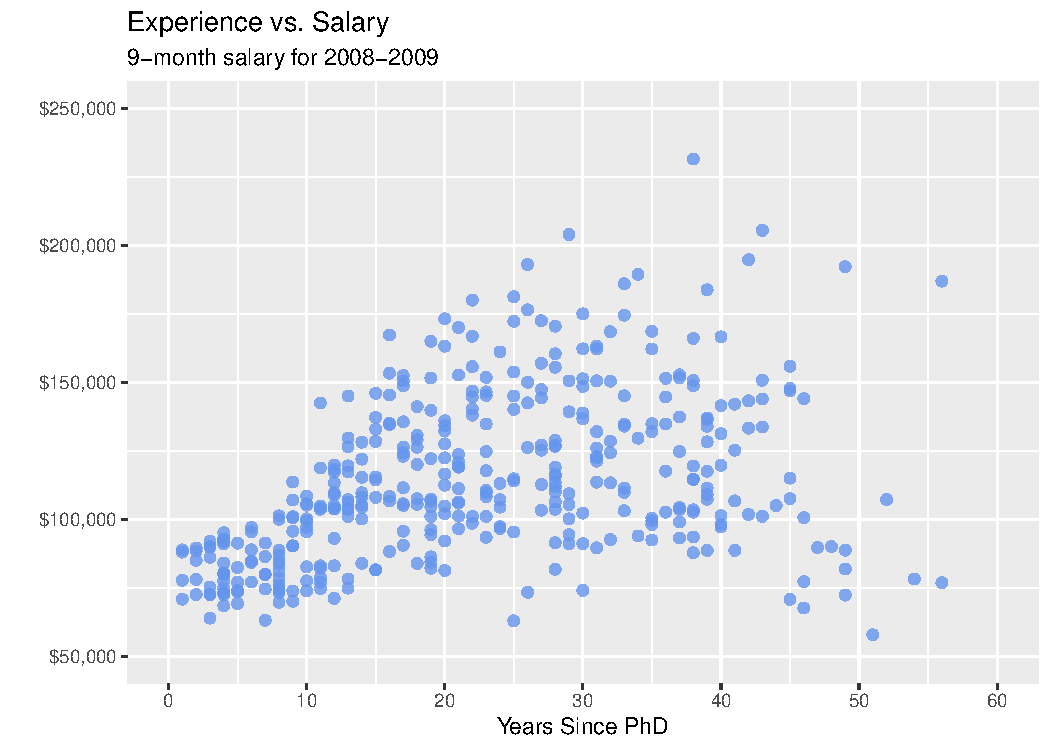
\includegraphics[width=.6\textwidth]{pics/plot1.1.pdf}		
\end{center}}
\end{frame}

\begin{frame}[fragile]{Scatterplot for 2D datasets + categorical variable}
	The scatterplot is the standard for representing continuous bivariate data.
	{\scriptsize
%<<plot1,fig.pos="t", fig.height=1, fig.width=1,fig.cap="">>=	
%	mlab <- "Manufacturing enterprises with 20 or more workers"
%	plab <- "Population size (1970 census) in thousands"
%	plot(popul ~ manu, data = USairpollution, xlab = mlab, ylab = plab)
\begin{center}
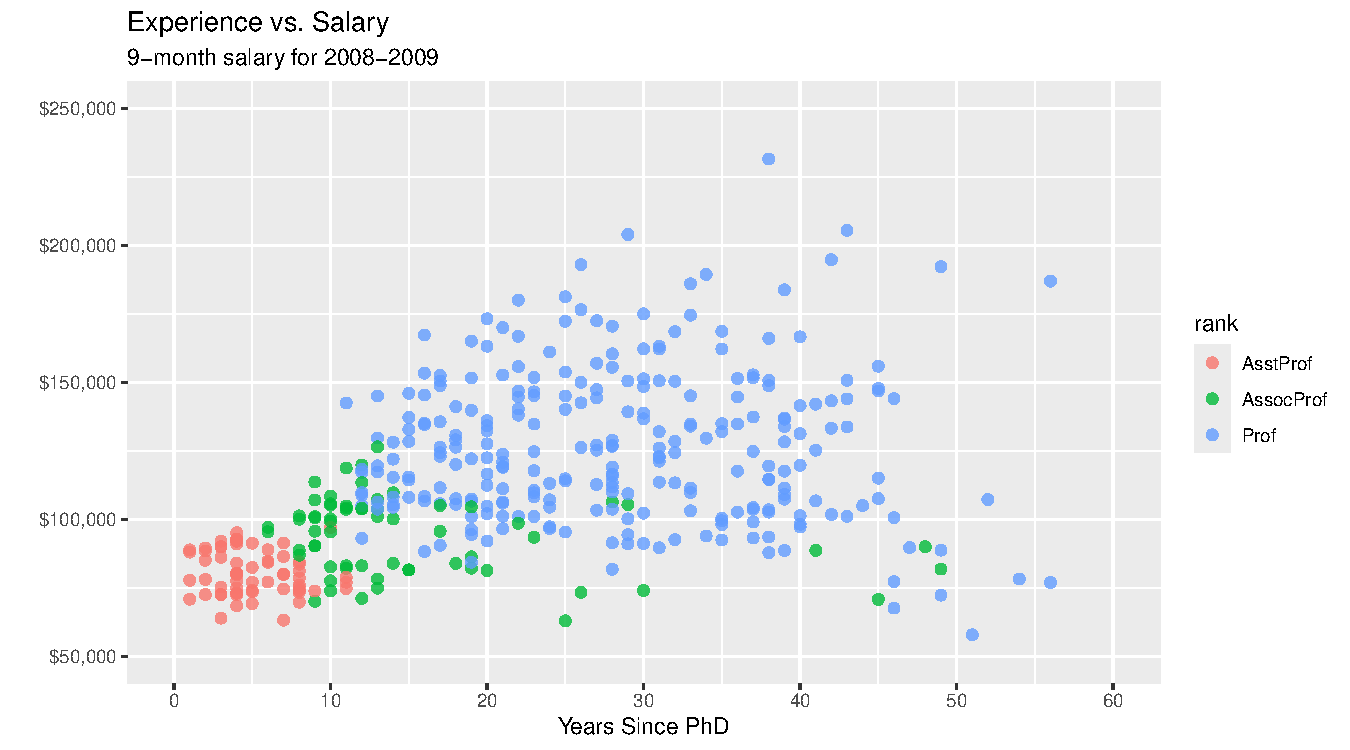
\includegraphics[width=.7\textwidth]{pics/plot1.2.pdf}		
\end{center}}
\end{frame}

\begin{frame}[fragile]{Scatterplot with some marginal information}
\begin{center}
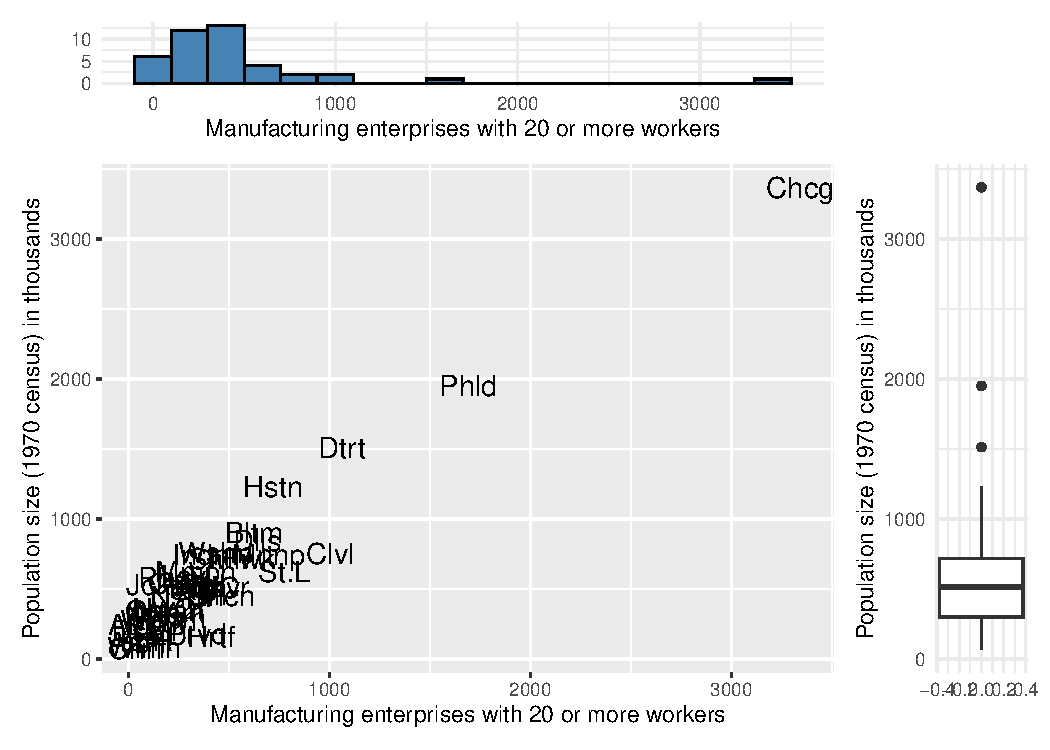
\includegraphics[width=.75\textwidth]{pics/plot1.3.pdf}		
\end{center}
\end{frame}


\begin{frame}[fragile]{2D kernel density estimation}
In our bigger gene expression dataset, take a look at differential expression between a wildtype and an FGF4-KO sample.

\tiny
\begin{Schunk}
\begin{Sinput}
> scp <- ggplot(dfx, aes(x = `59 E4.5 (PE)`,y = `92 E4.5 (FGF4-KO)`))
> plot1 <- scp + geom_point()
> plot2 <- scp + geom_point(alpha = 0.1)
> plot3 <- scp + geom_density2d(h = 0.5, bins = 60)
> library("RColorBrewer")
> colorscale = scale_fill_gradientn(colors = rev(brewer.pal(9, "YlGnBu")), 
+ 	values = c(0, exp(seq(-5, 0, length.out = 100))))
> plot4 <- scp + stat_density2d(h = 0.5, bins = 60,aes( fill = after_stat(level)), geom = "polygon") +  colorscale + coord_fixed()
\end{Sinput}
\end{Schunk}
\begin{center}
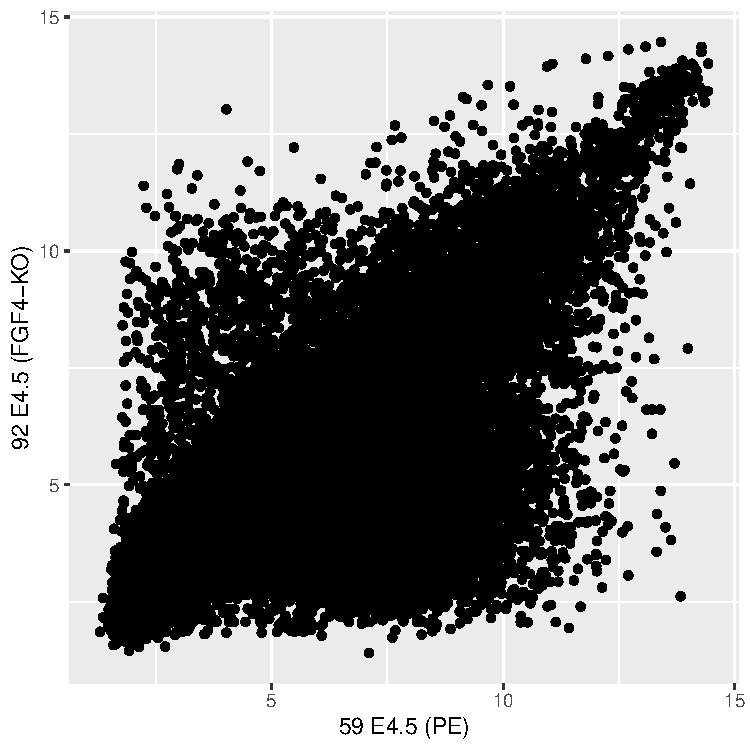
\includegraphics[height=3.2cm,width=3.2cm]{pics/plot1.5a.pdf}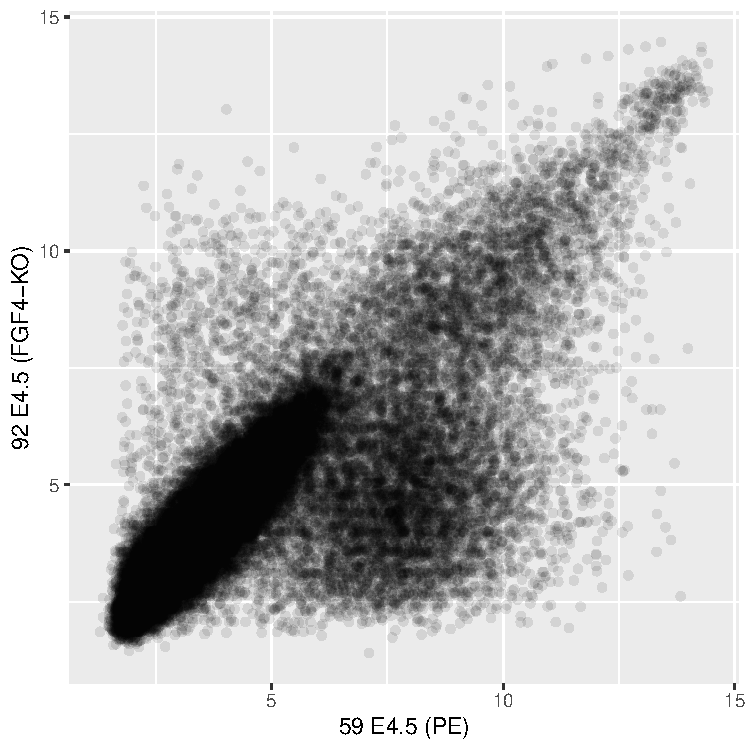
\includegraphics[height=3.2cm,width=3.2cm]{pics/plot1.5b.pdf}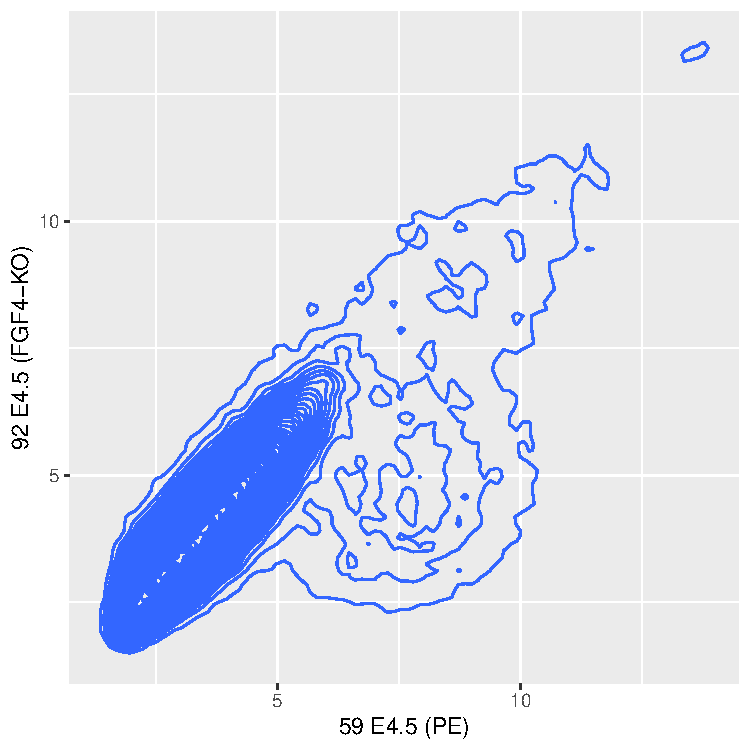
\includegraphics[height=3.2cm,width=3.2cm]{pics/plot1.5c.pdf}	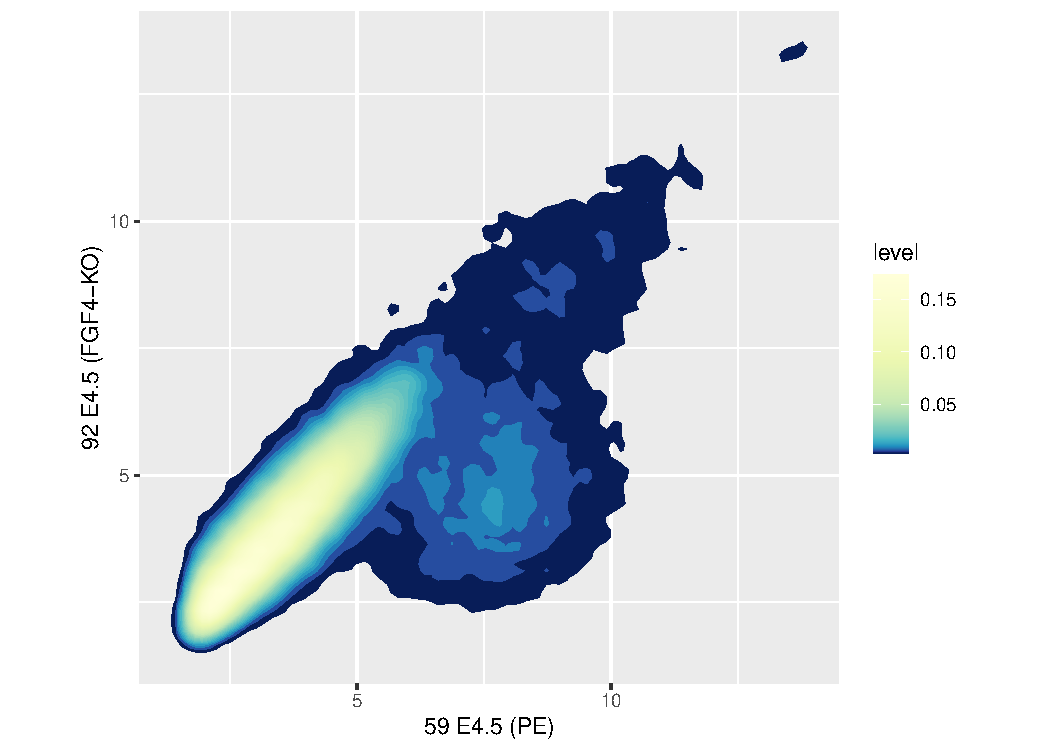
\includegraphics[height=3.2cm,width=4.3cm]{pics/plot1.5d.pdf}			
\end{center}
\end{frame}

\begin{frame}[fragile]{The scatterplot matrix and lattice plots}
%\scriptsize
\begin{center}
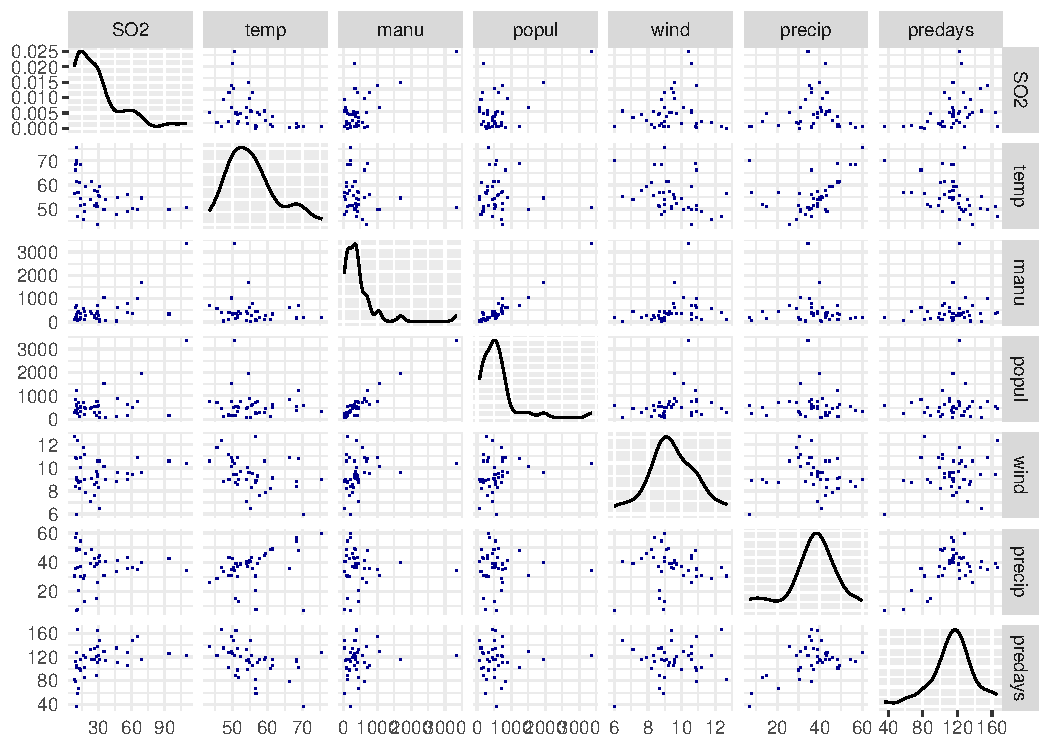
\includegraphics[width=.75\textwidth]{pics/plot1.4.pdf}		
\end{center}
\end{frame}



\begin{frame}[fragile]{The scatterplot matrix and lattice plots + 2D kernel density estimators}
%\scriptsize
\begin{center}
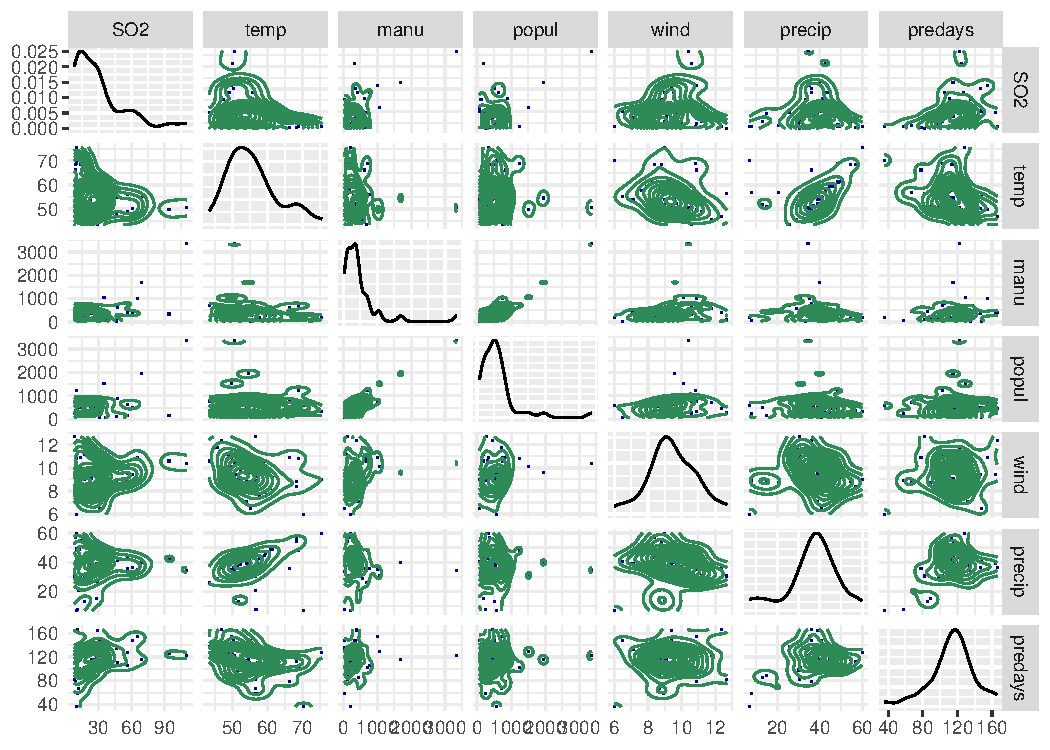
\includegraphics[width=.75\textwidth]{pics/plot1.6.pdf}		
\end{center}
\end{frame}




\begin{frame}[fragile]{Interactive graphics: Plotly}
Plotly is a powerful library for creating interactive, web-based visualizations. It's available in several programming languages including R and Python. With Plotly, users can create interactive plots like scatter plots, bar charts, heatmaps, and 3D plots.
\begin{Schunk}
\begin{Sinput}
> library(ggplot2)
> library(plotly)
> p <- ggplot(mpg, aes(x=displ, y=hwy, color=class)) + geom_point(size=3) + labs(x = "Engine displacement",
+ y = "Highway Mileage",color = "Car Class") + theme_bw()
> ggplotly(p)
\end{Sinput}
\end{Schunk}
Mousing over a point displays information about that point. Clicking on a
legend point, removes that class from the plot. Clicking on it again returns it.
Popup tools on the upper right of the plot allow you to zoom in and out of
the image, pan, select, reset axes, and download the image as a png file.
\end{frame}

\section{Notation and preliminaries (blackboard)}

\begin{frame}{Summary of this part}
	\begin{itemize}
		\item Vectors, matrices, random vectors
		\item Interpretations for $A\mathbf x$ and $AB$
		\item Linearity of expectation, bilinearity of covariance
	\end{itemize}
\end{frame}

\end{document}
